\subsection{Butterfly}{\label{pp:butterfly}}
\textbf{Problem Statement:}\\
Print the Butterfly pattern for a general $n$. See Starter code (below) for more details.
\begin{testcases}
	{$t$ \hfill(number of test cases, an integer)\\
	$n_1\ n_2\ \ldots\ n_t$ \hfill($t$ space seperated integers for each testcase)}
	{Butterfly pattern \hfill(each test case on a newline)}
	{$1 \leq n_i \leq 10$}
	{5\\1 2 3 4 5}
	% {*\space\space\space*\newline*\space*\space*}
	{\vspace{-2em}
	\begin{figure}[H]
	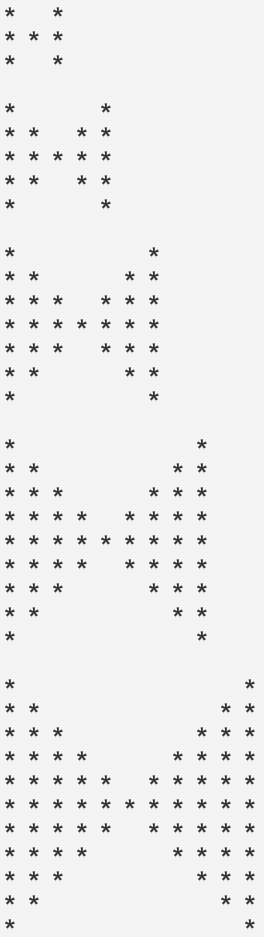
\includegraphics[width=0.23\linewidth]{Butterfly.png}
	\end{figure}
	}
	% \begin{table}[H]
	% \begin{tabular}{p{0.001pt}p{0.001pt}p{0.001pt}p{0.001pt}p{0.001pt}}
	% * &  &   &  & * \\
	% * &  & * &  & * \\
	% * &  &   &  & *
	% \end{tabular}
	% \end{table}
	% \begin{table}[H]
	% \begin{tabular}{lllll}
	% * &  &   &  & * \\
	% * &  & * &  & * \\
	% * &  &   &  & *
	% \end{tabular}
	% \end{table}
	{https://github.com/paramrathour/CS-101/tree/main/Starter Codes/Butterfly.cpp}
\end{testcases}
\begin{funvideo}
\href{https://youtu.be/fDek6cYijxI}{Chaos: The Science of the Butterfly Effect -- Veritasium}
\end{funvideo}